% !TEX encoding = UTF-8 Unicode
\documentclass[a4paper]{article}
%%%%%%%%%%%%%%%%%%%%%%%%%%%%%%%%%%%%%%%%%%%%%%%%%%%%%%%%%%%%%%%%%%%
% Packages using
%%%%%%%%%%%%%%%%%%%%%%%%%%%%%%%%%%%%%%%%%%%%%%%%%%%%%%%%%%%%%%%%%%%
\ifx\pdfoutput\undefined
\usepackage[dvips]{graphicx}
\DeclareGraphicsExtensions{.eps}
\else
\usepackage[pdftex]{graphicx}
\DeclareGraphicsExtensions{.pdf,.jpg,.png,.mps}
\pdfcompresslevel=9
\fi

\usepackage{color}
\usepackage{adjustbox}
\usepackage{enumitem}
\usepackage{xparse}
\usepackage[a4paper, total={6in, 8in}]{geometry}
\usepackage[numbers]{natbib}
\usepackage[utf8]{inputenc}
\usepackage[english]{babel}
\usepackage{indentfirst}
\addtolength{\topmargin}{-20mm}
\addtolength{\textheight}{70mm}
\usepackage{amsmath} % Added to get modern math environments
\usepackage{bm}
\usepackage{amssymb,amsfonts} %Added to get math
\usepackage{amsthm} % Added to get theorems
\usepackage{natbib} % Added to get better bibliography
\usepackage{soul} %underline
\usepackage{url}
% Special hack below to break the URL!
\def\UrlBreaks{\do\.\do\@\do\\\do\/\do\!\do\_\do\|\do\;\do\>\do\]%
	\do\)\do\,\do\?\do\'\do+\do\=\do\#\do\i\do\m\do\t\do\a\do\x}%
\urlstyle{rm} %
\usepackage[bookmarks=true,bookmarksnumbered=true,hypertexnames=true,breaklinks=true,colorlinks=true]{hyperref}
\hypersetup{
	pdfauthor = {Ubadigha Chinweze},
	pdftitle = {Information Retrieval and Processing--Setup of a Full Text System Implementing Automatic Metadata Extraction and Visualization},
	pdfsubject = {Set-Up Guide},
	pdfkeywords = {Django, Nginx, Postgres, Gunicorn, centOS 7}}

% Headers and footers (must be after the document settings)
\usepackage{fancyhdr} %Custom header package
\pagestyle{fancy} %Turn on fancy headers
\renewcommand{\headrulewidth}{0.4pt} %Header line
\renewcommand{\footrulewidth}{0.4pt} %Footer line

% Select what to do with todonotes: 
% \usepackage[disable]{todonotes} % notes not showed
\usepackage[draft]{todonotes}   % notes showed


%%%%%%%%%%%%%%%%%%%%%%%%%%%%%%%%%%%%%%%%%%%%%%%%%%%%%%%%%%%%%%%%%%%

\title{Step-by-step Procedure to Set Up Django with Postgres, Nginx, and Gunicorn on CentOS 7} 
%\author{Chinweze Ubadigha} 
\date{\today} 

\makeatletter
\def\step{%
	\@ifnextchar[ \@myitem{\@noitemargtrue\@myitem[\@itemlabel]}}
\def\@myitem[#1]{\item[#1]\mbox{}\\}
\makeatother


% Custom environments
\newenvironment{Step}{%
	\begin{enumerate}[label= \textbf {Step} \arabic*,align=left, leftmargin=1.0cm]%
	}{
\end{enumerate}%
}

\newenvironment{Thing}{%
	\begin{enumerate}[label=Thing \arabic*,align=left, leftmargin=1.0cm]%
	}{
\end{enumerate}%
}

\begin{document}
\maketitle

\section*{Introduction}
 \label{introduction}
Before we begin lets review briefly Django, Postgres, Gunicorn, Nginx and also why we chose to use these in
setting up our web server.  Django is a web framework which can be created using python application. Django
offers simplified development server but for anything slightly production related a more powerful and
secure web server is required \citenum{Digitalocea2016} . 
Django comes with default SQlite database but we will be using PostgreSQL a more powerful open source
object-relational database system instead \citenum{Thepostgresqlglobaldevelopmentgroup2016}. Thinking of security, NGINX is a free, open-source, high-performance HTTP server and reverse proxy . By reverse proxy, it enhances security and manages the web
traffic \citenum{Nginxincdoc2016}.\\ 
Gunicorn is an application server we will use to interface with our Django python applications and NGINX. Combining the features of these applications our Django web server will be security and performance enhanced. \par

\section* {Prerequisites}
\label{prerequisite}
Things you should have handy in order to complete this guide:

\begin{enumerate}
	\item CentOS 7 server.
	\item Sudo password (user should have sudo privileges).
	\item virtual environment. If you don't have any never mind, you will be guided on how to do that when the time comes.\\
\end{enumerate}

Lets get started,\\

\section* {Step by step procedure}
\begin{Step}
	\step
    \begin{minipage}[t]{\linewidth}
		\raggedright
		\adjustbox{valign=t}{%
			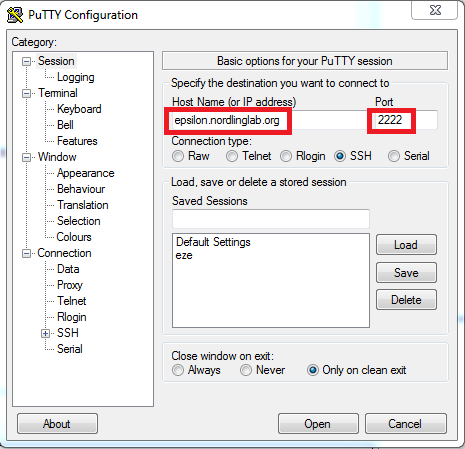
\includegraphics[width=.4\linewidth]{putty}
		}
		
		\medskip
		Login in to the server through putty using the following and as shown above.\\ %\autoref{fig:putty}:\\ \\
		Host name or IP address: \textbf{epsilon.nordlinglab.org}\\
		Port: \textbf{2222}\\
	\end{minipage}
	
%	\begin{figure}[h!]
%		\centering
%		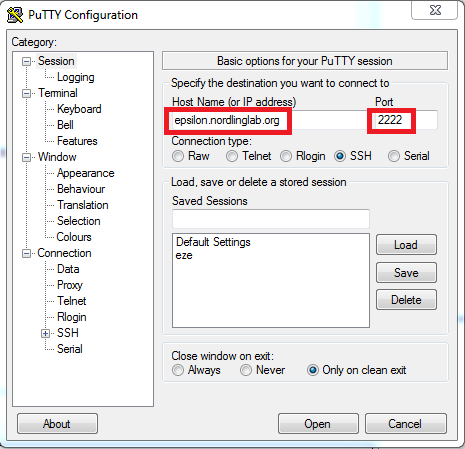
\includegraphics[scale=0.6]{putty}
%		\caption{putty login screen}
%		\label{fig:putty}
%	\end{figure}
	
	\step
	\begin{minipage}[t]{\linewidth}
		\raggedright
		\adjustbox{valign=t}{%
			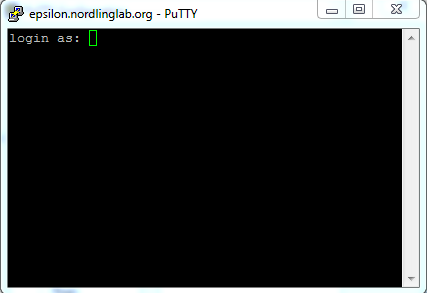
\includegraphics[width=.6\linewidth]{putty_screen}
		}
		
		\medskip
		A black screen will open as shown above. You will be prompted to key-in your \textbf{user name} followed by a \textbf{password}. Please do that.\\
	\end{minipage}		
\step
Now you've logged into the server. We will start right away to install the packages from EPEL and the
CentOS Repositories. Afterwards, we will use Python package manager \textbf{\textit{pip}} to install some
additional components.\\ Type the following in the command window to enable EPEL repository. When prompted
for the sudo password please type it.\\ \\
\textbf{\emph{sudo yum install epel-release}}\\ \\
With the new repository available, we can install all we needed in one command.
\step
Type the following into the command window:\\ \\
\textbf{\emph{sudo yum install python-pip python-devel postgresql-server postgresql-devel postgresql-contrib gcc nginx}}\\ 
\step
Configure and Start PostgreSQL. First, initialize the PostgreSQL database. We can do that by typing:\\ \\
\textbf{\emph{sudo postgresql-setup initdb}}\\
\step
Start the PostgreSQL service by typing:\\ \\
\textbf{\emph{sudo systemctl start postgresql}}\\
\step
Change the authentication method for the database to allow our Django instance user to have access using password. Type the following to edit using \textbf{nano} editor. Remember when prompted for password please type it.\\ \\
\textbf{\emph{sudo nano /var/lib/pgsql/data/pg\_hba.conf}}\\
\step
\medskip When the file opens, move to the bottom of the page and edit the file as shown below. Modify the two host lines by changing the last column (the authentication method) to \textbf{md5}. This will allow password authentication:\\
\begin{minipage}[t]{\linewidth}
	\raggedright
	\adjustbox{valign=t}{%
		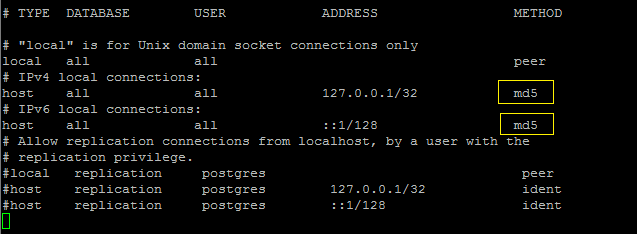
\includegraphics[width=1.0\linewidth]{post_auth}
	}\\
	
	\medskip
	When you are finished, save and close the file by clicking \textbf{ctrl C} followed by \textbf{"Y"} and then \textbf{"Enter"}. \\
\end{minipage}

\step
Restart the service and also enable the PostgreSQL so that it start automatically at boot:\\ \\
\textbf{\emph{sudo systemctl restart postgresql}}
\textbf{\emph{sudo systemctl enable postgresql}}\\
\step
It will be convenient to change to root user temporarily in order to work with postgres locally. Type\\ \\
\textbf{\emph{sudo su - postgres}}\\ \\followed by\\ \\
\textbf{\emph{psql}}\\ \\
This will be give you a PostgreSQL prompt where we can set up our requirements.\\

\step
Creat a database for our project:\\ \\
\textbf{\emph{CREATE DATABASE \textcolor{red}{myproject};}}\\ \\
Next create database user for our project:\\ \\
\textbf{\emph{CREATE USER \textcolor{red}{myprojectuser} WITH PASSWORD '\textcolor{red}{password}';}}\\ \\
Give our new user access to administer our new database:\\ \\
\textbf{\emph{GRANT ALL PRIVILEGES ON DATABASE \textcolor{red}{myproject} TO \textcolor{red}{myprojectuser};}}\\ \\
Notice all the command must end with semicolon. When you are done exit the postgreSQL promtp by typing:\\ \\
\bm{$\backslash q$}\\ \\
Now also exit the root user by typing:\\ \\
\textbf{\emph{exit}}\\

\step
We now create our python virtual environment for your Django Project. If you already have virtualenv installed you skip this step, else type:\\ \\
\textbf{\emph{sudo pip install virtualenv}}\\ \\ \\

\step
Make a directory for you project and navigate into the directory:\\ \\
\textbf{\emph{mkdir $\sim$/\textcolor{red}{myproject}}}\\ \\
\textbf{\emph{cd $\sim$/\textcolor{red}{myproject}}}\\ \\

\step
Within the project directory, create python virtual environment by typing:\\ \\
\textbf{\emph{virtualenv ~/\textcolor{red}{myprojectenv}}}\\ \\
Activate the virtual environment:\\ \\
\textbf{\emph{source ~/\textcolor{red}{myprojectenv}/bin/activate}}

\step
With virtual environment activated, proceed to install Django, gunicorn and the psycopg2 PostgreSQL adaptor with the local instance of \textit{pip}:\\ \\
\textbf{\emph{pip install django gunicorn psycopg2}}\\ \\

\step
Create Django Project file in the same directory:\\ \\
\textbf{\emph{django-admin.py startproject \textcolor{red}{myproject}}}\\ \\

\step
Open the django project files settings\\ \\
\textbf{\emph{nano \textcolor{red}{myproject}/settings.py}}\\ \\
Change the settings with your PostgreSQL database information. We have to give the database name, database username, the database username's password and then specify that the database is located on the local computer as shown below:\\ \\
\begin{minipage}[t]{\linewidth}
	\raggedright
	\adjustbox{valign=t}{%
		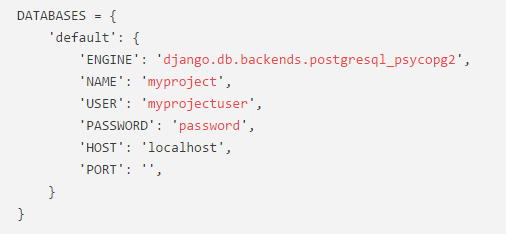
\includegraphics[width=0.9\linewidth]{django_db}
	}\\
\end{minipage}

\step
Next, move to the bottom of the file and add where the static files should be placed. This is so Nginx could handle request for these items:\\ \\
\textbf{\emph{STATIC\_ROOT = os.path.join(BASE\_DIR, "static/")}}\\ \\
Save and close the the file when you are done.\\ \\ \\

\step
migrate the initial database schema to our PostgreSQL database using the management script:\\ \\
\textbf{\emph{ cd $\sim$/\textcolor{red}{myproject}}}\\ \\
\textbf{\emph{./manage.py makemigrations }}\\ \\
\textbf{\emph{./manage.py makemigrate}}\\ \\
Create an administrative user for the project by typing:\\ \\ 
\textbf{\emph{./manage.py createsuperuser}}\\ \\
When prompted select a \textit{\textbf {username}}, provide an \textit{\textbf {email address}}, and choose and confirm a \textit{\textbf {password}}.

\step
collect all of the static content into the directory location we configured by typing:\\ \\
\textbf{\emph{./manage.py collectstatic}}\\ \\
When prompted to confirm the operation type \textbf{"Y"}\\\\

\step
Finally, you can test your project by starting up the Django development server with this command:\\ \\
\textbf{\emph{./manage.py runserver 140.116.155.13:8000}}\\ \\
In your web browser, visit your server's \textbf{domain name} or \textbf{IP address} followed by \textbf{:8000}:\\\\
\textbf{\emph{http://\textcolor{red}{140.116.155.13}:8000}}\\ \\

\step
You should see the following page, if everything is properly configured:\\ \\
\begin{minipage}[t]{\linewidth}
	\raggedright
	\adjustbox{valign=t}{%
		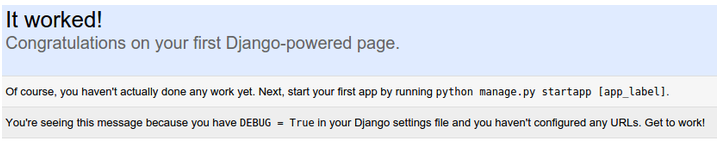
\includegraphics[width=1\linewidth]{django_df}
	}
\end{minipage}
\medskip \ \\
	if you append \textbf{/admin} to the end of the url in the address bar, you will see the following. Input the \textbf{username} and \textbf{password} you created as \textbf{superuser}:
	
\begin{minipage}[t]{\linewidth}
	\raggedright
	\adjustbox{valign=t}{%
		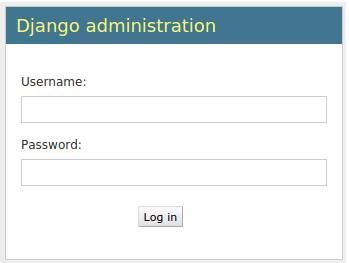
\includegraphics[width=0.4\linewidth]{django_admin}
	}
\end{minipage}
	\medskip \ \\	
	After authenticating, you can access the default Django admin interface:\\\\
\begin{minipage}[t]{\linewidth}
		\raggedright
		\adjustbox{valign=t}{%
			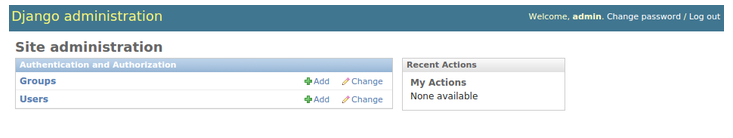
\includegraphics[width=0.8\linewidth]{django_int}
		}
\end{minipage}
	\medskip \ \\
	When you are finished exploring, hit \textbf{CTRL-C} in the terminal window to shut down the development server.

\step
Test the Gunicorn's ability to serve the project :\\ \\
\textbf{\emph{ cd $\sim$/\textcolor{red}{myproject}}}\\ \\
\textbf{\emph{ gunicorn --bind 0.0.0.0:8000 $\sim$/\textcolor{red}{myproject}.wsgi:application}}\\ \\

Hit \textbf{CTRL-C} to stop Gunicorn.\\\\
Type the following to get out of our virtual environment:\\\\
\textbf{\emph{ deactivate}}\\ \\

\step
Create and open a Systemd service file for Gunicorn with sudo privileges:\\ \\
\textbf{\emph{sudo nano /etc/systemd/system/gunicorn.service}}\\ \\
Input the following inside the file:\\\\
\textbf{\emph{[Unit]}}\\
\textbf{\emph{Description=gunicorn daemon}}\\
\textbf{\emph{After=network.target}}\\ \\
\textbf{\emph{[Service]}}\\
\textbf{\emph{User=\textcolor{red}{user}}}\\
\textbf{\emph{Group=nginx}}\\
\textbf{\emph{WorkingDirectory=/home/\textcolor{red}{user}/\textcolor{red}{myproject}}}\\
\textbf{\emph{ExecStart=/home/\textcolor{red}{user}/\textcolor{red}{myproject}/\textcolor{red}{myprojectenv}/bin/gunicorn --workers 3 --bind unix:/home/\textcolor{red}{user}/\textcolor{red}{myproject}/\textcolor{red}{myproject}.sock \textcolor{red}{myproject}.wsgi:application}}\\ \\
\textbf{\emph{[Install]}}\\
\textbf{\emph{WantedBy=multi-user.target}}\\

Note the bars \textbf{"|"} in front of \textit{"workers"} and \textit{"bind"} are two and no space between them.\\
Save and close the the file when you are done, \textbf{CTRL-C} and \textbf{"Y"}\\\\

\step
We now start the Gunicorn we created and enable it so that it starts at boot:\\ \\
\textbf{\emph{ sudo systemctl start gunicorn}}\\
\textbf{\emph{ sudo systemctl enable gunicorn}}\\

\step
We will now configure Nginx to proxy pass to Gunicorn i.e pass traffic to the process. We do this by modifying the Nginx configuration file. To learn more on how Nginx works or being configured see \citenum{Nginxincconfig2016}:\\ \\
\textbf{\emph{ sudo systemctl start gunicorn}}\\ \\
To do this open the Nginx configuration file:\\\\
\textbf{\emph{sudo nano /etc/nginx/nginx.conf}}\\

Inside, open up a new server block just above the server block that is already present as shown in the below (red text):\\\\

\begin{minipage}[t]{\linewidth}
	\raggedright
	\adjustbox{valign=t}{%
		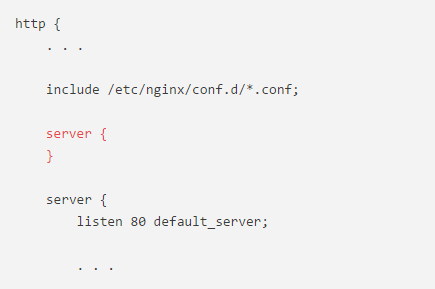
\includegraphics[width=0.8\linewidth]{nginx_bl}
	}
\end{minipage}
\medskip \ \\
Insert the following code into the server block as shown below. Make sure to substitute accordingly the red texts:\\

\begin{minipage}[t]{\linewidth}
	\raggedright
	\adjustbox{valign=t}{%
		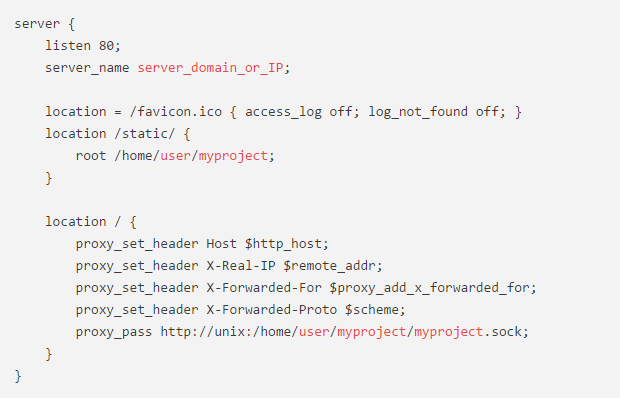
\includegraphics[width=1\linewidth]{nginx_lo}
	}
\end{minipage}
\medskip \ \\

Save and close the file when you are done.

\step
Add the nginx user to your group with the following command. Substitute your own \textbf{\textcolor{red}{username}} for the \textbf{\textcolor{red}{user}} in the command:\\ \\\\
\textbf{\emph{ sudo usermod -a -G \textcolor{red}{user} nginx}}\\\\\\

Give our user group execute permissions on our home directory. This will allow the Nginx process to enter and access content within:\\\\
\textbf{\emph{chmod 710 /home/\textcolor{red}{user} nginx}}\\\\

Test the Nginx configuration file for syntax errors:\\\\
\textbf{\emph{sudo nginx -tx}}\\

If no errors are present, restart the Nginx service by typing:\\\\
\textbf{\emph{sudo systemctl start nginx}}\\

Tell the system to start the Nginx server at boot by typing:\\\\
\textbf{\emph{sudo systemctl enable nginx}}\\

If everything went well you should now have access to your Django application in your browser over your server's domain name or IP address without specifying a port.\\

You have successfully setup a Django webserver that runs with PostgreSQL, Gunicorn and Nginx.

\end{Step}

	%%%%%%%%%%%%%%%%%%%%%%%%%%%%%%%%%%%%%%%%%%%%%%%%%%%%%%%%%%%%%%%%%%%
	% References
	% Using Mendeley Desktop with library.bib
	%%%%%%%%%%%%%%%%%%%%%%%%%%%%%%%%%%%%%%%%%%%%%%%%%%%%%%%%%%%%%%%%%%%	
	\newpage	
	\bibliographystyle{IEEEtran}
	\bibliography{library}	
	\clearpage 

\end{document}